\section{INTRODUCTION}
This chapter covers an overview of the existing location based positioning solutions  with location services, feasibility of proposed solution, requirement gathering techniques, requirement analysis, goals of the research project and the limitations, functional and non-functional requirements.

\section{REQUIREMENT GATHERING TECHNIQUES}
In any system, gathering exact,accurate requirement is really important to get right outcome from the system. Therefore, requirement gathering phase is one of the most important phases of software development life-cycle. It leads to the success of entire project.
	\paragraph{}
	In this project, requirement gathering has been done by reviewing of  existing systems and identifying areas that have to be improved.


\section{SIMILAR SYSTEMS}
There are many approaches introduced to overcome problems related to system authentication. But still hackers manage to gain access to the systems by using vulnerability of the authentication process. Even most powerful authentication methods are still fail due to bad practices or incomplete/ incorrect implementation. There are some researches available which address the same issue with different types of solutions. Most of the researches have been done to authenticate the user by using user's GPS(Global Position Service) coordinates. But it seems that this method cannot be applied always due to poor GPS signal strengths and GPS coordination values which are highly dependent on weather conditions such as clouds and wind. Also the accuracy level of the GPS coordinates within the buildings/covered areas are significantly low. 

\paragraph{}
This suggested approach uses Wi-Fi access point's signal strength to locate the user location according to the Wi-Fi access point. By considering the Wi-Fi signal strength together with valid user name and password, system authentication rules can be defined to allow or deny access to the user.

\subsection{PHILIPS INDOOR POSITIONNING SYSTEM}
Since Lite Emitted Diode (LED) fixtures deliver high-quality light with energy-efficiency, this approach uses Philips Visible Light Communication (VLC) which is patented by Philips to communicate with cameras and smart phones. This solution consists with special software with cloud infrastructure, it is possible to locate the precise position of the customer inside the shop up to 30cm accuracy.\cite{philips}

\paragraph{}
This is how this method works.\cite{philips_3}
	\begin{enumerate}
		\item  Store lighting acts as an indoor positioning infrastructure. Indoor positioning system works with LED luminaires that are embedded with VLC technology. 
		\item VLC sends out a unique code from each light fixture to the mobile device.
		\item Mobile device's camera detects the code and the phone revels its position.
		\item Location is identified and location based service is delivered to the mobile device.
	\end{enumerate}
		\begin{figure*}[h]	
			\centering
			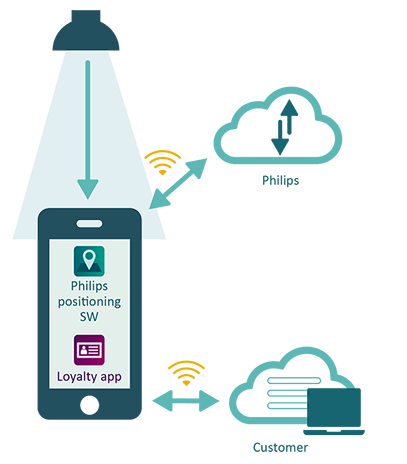
\includegraphics[width=0.5\textwidth]{philips.png}
			\caption{Philips indoor positioning system}
		\end{figure*}

\newpage
\paragraph{}
Disadvantages of the system
	\begin{itemize}
		\item Have to use specially designed LED bulbs with embedded VLC technology
		\item This method is used for promotions which may not be relevant to the customer or choice of the customer since method does not use any analysis information about customer's previous information
		\item No user authentication mechanism is available and any user with the mobile application can use the information
	\end{itemize}

\subsection{INDOO.RS - INDOOR POSITIONING SYSTEM}
This method uses "Trilateration Technique" to pinpoint a location inside a building. Real time data is derived from mix of the following.
	\begin{itemize}
		\item iBeacon Protocol \cite{iBeacons}
			\subitem iBeacon is the name for Apple's technology standard. This allows both Android and iOS devices to listen for signals from beacons and react accordingly. iBeacons allows mobile applications to be aware of its position on a micro-local scale. Bluetooth Low Energy (BLE) technology has been used to communicate between iBeacons and mobile devices.
		\item Senser Fusion
		\item SLAM Engine technology\cite{slam_eng}
	\end{itemize}

\paragraph{}
Disadvantages of the system
\begin{itemize}
	\item Special devices should be used such as iBeacons to locate the position.
	\item This method just provides the location of user and it does not involve in authenticating the user.
	\item Includes additional cost due to special devices required.
	
\end{itemize}


\section{FUNCTIONAL AND NON-FUNCTIONAL REQUIREMENTS}
\subsection{FUNCTIONAL REQUIREMENTS}
\begin{itemize}
	\item Authorized users should be able to connect to the access point only when they are in a position which is allowed by administrator.
	\item Authorized users those who are outside from the allowed area, but have valid user name and password are still not allowed to connect to access point.
\end{itemize}

\subsection{NON-FUNCTIONAL REQUIREMENTS}
\begin{itemize}
	\item Authentication
	\begin{itemize}
		\item Authentication should be done not only with valid user name and password, but also location information according to the Wi-Fi signal strength.
	\end{itemize}
	\item Authorization
	\begin{itemize}
		\item Only authorized parties allow to make modifications, changes to the system.
	\end{itemize}
	\item Availability
	\begin{itemize}
		\item The system should be available in any time whenever user needs to use it.
	\end{itemize}

	\item Reliability
	\begin{itemize}
		\item The system should function without defect under defined conditions/ environment and specific period of time.
	\end{itemize}
	
	\item Usability /User friendliness
	\begin{itemize}
		\item The system should be able to use without extra effort and GUI also need to be easy for the user.
	\end{itemize}
	
	\item Stability
	\begin{itemize}
		\item Application should be stable and all components should function smoothly.
	\end{itemize}
	
\end{itemize}